\documentclass[conference]{IEEEtran}
%\usepackage{cite}
\usepackage[dvips]{graphicx}
 \DeclareGraphicsExtensions{.eps}
%\usepackage[cmex10]{amsmath}
\usepackage[tight,footnotesize]{subfigure}

\begin{document}

\title{An RFID Interface for 3D Audio Web Consumption}
\author{
\IEEEauthorblockN{Victor K.Y. Wu}
\IEEEauthorblockA{Department of Electrical and Computer Engineering\\
University of Illinois at Urbana-Champaign\\
Email: vwu3@illinois.edu}
\and
\IEEEauthorblockN{Roy H. Campbell}
\IEEEauthorblockA{Department of Computer Science\\
University of Illinois at Urbana-Champaign\\
Email: rhc@illinois.edu}

}
\maketitle

\section{Introduction}
We propose a novel multi-stream audio web consumption system using a passive UHF RFID interface.  For example, in an eyes-free setting such as an in-vehicle audio system, the left speaker quietly streams the subject lines of a user's unread emails.  Simultaneously, the user chats through a VOIP (voice over Internet protocol) connection via a microphone and the right speaker.  On a dedicated surface on the vehicle dashboard, several RFID tags are attached, where an interrogator scans for tags.  When it is safe to do so, the user rearranges the tags (possibly removing or adding tags), creating a new session where she can consume other web content in 3D audio space.  In another scenario, a user consumes multi-stream audio web content via a mobile device.  She uses an integrated interrogator in the device to scan NFC (near field communication) tags, customizing her web consumption experience.  The NFC tags may be part of smart posters or displays, or might be even carried by the user herself.

In the rest of this work, we provide details of our proposed system.  We also present a preliminary system prototype.

\section{Eyes-free 3D audio}
Many situations prevent users from accessing the web through a predominantly visual interface.  Obviously, sightless users fall into this category.  Additionally, scenarios such as driving, jogging, or standing in a crowded subway train do not allow a user to focus on some sort of display.  These are known as eyes-free settings.  Furthermore, we argue that in many situations where visual attention is perhaps plausible, it is not necessarily safe, and does not provide a rich Internet experience.  We therefore propose accessing web content through a predominantly audio interface aided by RFID tags (explained in more detail in the next section).  We fully exploit the 3D audio space to allow users to possibly consume multiple streams of content simultaneously.  That is, each sound source (corresponding to a particular web service, for example), is virtually placed at a particular location in 3D audio space, relative to the user's head.  Closer sounds are louder, and the content in certain directions are more easily focused on, as shown in previous literature \cite{2009Vazquez-Alvarez}.  Depending on the application, we propose moving the sound sources and (and even the user) dynamically in the virtual space.  For example, suppose a social networking web service is streaming audio updates to the user in the audio space in front of her head (where it is easy to listen to).  If a critical situation arises (such as her bank detecting possible credit card fraud, or the weather authorities detecting an approaching storm), the social stream would be pushed behind to the back of the user's head.  And then an appropriate stream (automatic phone call to the bank or storm tracker updates) would be pushed to the front, enabling the user to attend to the critical information.

\section{RFID interface}
We propose using RFID tags as the main input interface for our 3D audio web consumption system.  In a simple (yet very intuitive), first-order design, each RFID tag represents a particular web service.  If a user brings a tag within the interrogator's range, the associated web service becomes accessible in the user's 3D audio space.  Other more elaborate designs include finer granularity customization and control.  For example, one particular tag may represent an email web service which only streams subject lines by default.  Other tags are used to further navigate within the email system, such as opening and reading messages, or archiving messages in specific folders.

RFID tags benefit from being a simple input interface.  They are easily manipulated in eyes-free scenarios.  Additionally, they allow for a very flexible, extendable, and transferrable system.  That is, users can easily acquire new tags (even trading amongst themselves), depending on the various application scenarios.  For example, consider a social networking web service that allows users to customize which contacts they want to receive updates from.  A user initially stores individual contacts or contact groups inside tags by scanning (and writing to) them.  When a tag is scanned later by the system interrogator, the associated contacts' updates are streamed to her.  Later, she can readjust the contacts if so desired.

RFID tags have steadily increased in storage capacity \cite{web:Tego}, allowing for even more possibilities in our proposed system.  In particular, tags serve to also store content itself.  For example, a set of tags in the scan range of an interrogator can buffer incoming web data, to allow the user an uninterrupted experience, even if network connectivity is irregular.

In our proposed system, we focus on passive UHF RFID technology, due to it's robust ability to scan multiple tags efficiently.  However, related technologies such as NFC may also be applicable in certain scenarios.  (Nonetheless, the underlying ideas of using such a wireless tag-based interface remain the same.)  For example, consider a user carrying multiple NFC tags.  These may possibly even be sewn directly into clothing, or worn as attachments (bracelet, necklace, etc.)  The user has a mobile phone with an integrated NFC interrogator (which is already commercially available \cite{web:NFC}.  There has also been work in integrating RFID interrogators into phones \cite{2009Savolainen}).  The user easily scans the worn NFC tags with her device, with simple hand gestures.  This creates a dynamic interface for 3D audio
web consumption.  For example, scanning tag A, followed by tag B may initiate a web service to stream current stock prices.  Scanning tag B, and then tag A initiates not only the stock prices stream, but also a simultaneous stream of financial news headlines.  These two choices are readily achieved by two opposing hand gestures while holding the device.

\section{Preliminary System Prototype}
We provide a preliminary software prototype of our ideas.  We use an Alien ALR-9650 RFID interrogator connected to a laptop running our software application.  The application continually communicates with the reader, knowing which RFID tags are currently being interrogated.  Eight tags correspond to the following eight respective web content streams:  a song, an email service, a Facebook news feed, a Twitter feed, a set of sports scores, a set of stock prices, a weather report, and a set of world news headlines.  (These are simulated with pre-generated audio files stored on the laptop.)  A user listens to the audio files with headphones.  The application plays the audio files corresponding to the tags in the scan range of the interrogator, for up to to five tags, in 3D audio space.  As tags are added and removed, the audio is changed accordingly.  We use OpenAL, a 3D audio library to position the sound sources.

We detail how the sound sources are dynamically located in 3D audio space.  Assuming the user is looking straight forward, the locations are always on the 2D plane of the user's head, where the plane is parallel to the ground plane.  Then each location can be characterized by the distance from the user's head, and the angle it sweeps out.  We first consider the angles.  Taking $0^{\circ}$ as the direction of the user looking straight forward, and positive angles sweeping to her left, Table \ref{angles} details the angles of sound source locations, depending on the number of sounds playing.
\begin{table}[h]
\begin{center}
  \begin{tabular}{ c | l }
   number of sounds & angles \\ \hline 
    $1$ & $0^{\circ}$ \\ \hline
    $2$ & $270^{\circ}, 90^{\circ}$ \\ \hline
    $3$ & $0^{\circ}, 270^{\circ}, 90^{\circ}$ \\ \hline
    $4$ & $0^{\circ}, 288^{\circ}, 72^{\circ}, 216^{\circ}$ \\ \hline
    $5$ & $0^{\circ}, 288^{\circ}, 72^{\circ}, 216^{\circ}, 144^{\circ}$  
  \end{tabular}
 \end{center}
 \label{angles}
\end{table}
The angles are ordered according to how long (in increasing time) corresponding tags have been in the range of the interrogator.  For example, if there are three tags, the newest arriving one's associated sound is located at $0^{\circ}$, the middle one at $270^{\circ}$, and the oldest one at $90^{\circ}$.  The distance of each sound source from the user's head scales with the time it's associated tag has been in the scan range.  That is, newer tags are closer.  Intuitively, when a user is interested in listening to a new web stream, she places the associated tag in the interrogator's scan range, and that web stream is most easily attended to, from an audio perception point of view.  Older web streams are pushed further away in 3D audio space.  (Note that when a tag leaves the scan range, and returns later, it's time in the scan range is reset to zero.  That is, it is treated as a newly arriving tag.)  When more than five tags are placed in the scan range, only the five newest tags' sounds are streamed.  Also, the angles are designed such that the newer sound sources are located in front of the user's head, again allowing for easier focus \cite{2009Vazquez-Alvarez}.

Fig. \ref{figure} shows a screenshot of our application displaying the current sound sources playing in 3D audio space.  We see that the user has just placed the tag corresponding to stock prices in the interrogator scan range.  Stock prices are therefore directly streaming in front of the user's head at a close distance.  The Facebook news feed and sports scores sounds are a bit further away, showing that their associated tags were placed in the scan range previously.  The email service and song are even further away.  The song tag thus has been in the scan range the longest (among these five tags).  
\begin{figure}
\centering
\includegraphics[clip=true, viewport=0 100 600 700, width=3in]{program.eps}
\caption{Sound sources in 3D audio space.\label{figure}}
\end{figure}

\section{Conclusion and Future Directions}
In this work, we propose a novel multi-stream audio web consumption system using a passive UHF RFID interface.  We provide a working system prototype to demonstrate our ideas.  In the future, we aim to develop more dynamic interfaces using RFID tags, allowing more flexibility and control for the user, thus providng a much richer web consumption experience.

\begin{thebibliography}{1}

\bibitem{2009Vazquez-Alvarez}
Y. Vazquez-Alvarez and S. Brewster, ``Investigating Background \& Foreground Interactions Using Spatial Audio Cues," in \emph{Proc. 2009 ACM Conference on Human Factors in Computing Systems (CHI)}, Boston, MA, Apr. 2009, pp. 3823-3828.

\bibitem{web:Tego}
``TegoChip." Tego. [Online]. Available: http://www.tegoinc.com/chips.htm 

\bibitem{web:NFC}
``NFC Research: Devices," in \emph{Near Field Communications Research Lab}.  [Online].  Available: http://www.nfc-research.at/index.php?id=45

\bibitem{2009Savolainen}
J.T. Savolainen, H. Hirvola, and S. Iraji, ``EPC UHF RFID Reader: Mobile Phone Integration and Services," in \emph{Proc. 2009 IEEE Consumer Communications and Networking Conference (CCNC)}, Las Vegas, NV, Jan. 2009.


\end{thebibliography}

\end{document}
